\documentclass[12pt,a4paper]{article}

% ---------------------------------------------------------------------------
% Preambulo
% ---------------------------------------------------------------------------
\usepackage[utf8]{inputenc}
\usepackage[T1]{fontenc}
\usepackage{lmodern}
\usepackage[brazilian]{babel}
\usepackage{csquotes}
\usepackage[a4paper,top=3cm,bottom=2cm,left=3cm,right=2cm]{geometry}
\usepackage{graphicx}
\usepackage{booktabs}
\usepackage{longtable}
\usepackage{array}
\usepackage{caption}
\usepackage{float}
\usepackage{tikz}
\usetikzlibrary{positioning,arrows.meta}
\usepackage[colorlinks=true,linkcolor=black,citecolor=black,urlcolor=blue]{hyperref}

\captionsetup{labelsep=endash,justification=centering,font=small}
\captionsetup[table]{position=top}
\captionsetup[figure]{position=bottom}

\usepackage[backend=biber,style=abnt]{biblatex}
\addbibresource{references.bib}

\title{Manutenção predial sustentável em edificações públicas/universitárias: critérios, métodos multicritério e lacunas de apoio à decisão no ambiente construído}
\author{Adinailson Guimarães de Oliveira \\ Programa de Pós-Graduação em Biossistemas, Universidade Federal do Sul da Bahia (UFSB)}
\date{}

% ---------------------------------------------------------------------------
% Documento
% ---------------------------------------------------------------------------
\begin{document}

\maketitle

\noindent\textit{Rascunho de trabalho -- título sujeito a ajuste após consolidação da discussão. Preparado para compilação em \LaTeX{} conforme estrutura e norma de citação (ABNT) exigidas pela revista MIX Sustentável (ISSN 2447-3073).}

\bigskip

\begin{center}
\textbf{Resumo}
\end{center}

\noindent Este artigo tem como objetivo identificar como a literatura científica integra sustentabilidade, manutenção e gestão de edificações e métodos de apoio multicritério à decisão, e em que medida essa integração oferece bases para priorizar intervenções em edificações públicas universitárias. Para isso, foi conduzida uma revisão integrativa sistematizada, com apoio bibliométrico em três bases (Scopus, Web of Science e Crossref, 2010--2026) e síntese temática apoiada em título, resumo e palavras-chave, sem leitura de texto completo, resultando em um núcleo final de 104 registros após triagem, auditoria qualitativa e reavaliação criteriosa. Os resultados indicam predominância de critérios técnico-operacionais e institucionais de sustentabilidade sobre critérios ambientais, econômicos e sociais explicitamente nomeados, além de maior frequência de instrumentos genéricos de apoio à decisão (\textit{framework}, \textit{decision support}, BIM) do que de métodos multicritério formalmente nomeados (AHP, TOPSIS, MCDM), ainda minoritários no núcleo final. A aplicabilidade a instituições públicas de ensino superior permanece pouco explorada no corpus internacional sistematizado, com lacuna específica identificada em 11,5\% dos registros do núcleo final, o que sustenta a proposição de uma matriz analítica orientada a investigações futuras, não uma solução já consolidada pela literatura.

\medskip
\noindent\textbf{Palavras-chave:} manutenção predial; sustentabilidade; métodos multicritério de decisão; gestão de edificações públicas; ambiente construído.

\bigskip

\begin{center}
\textbf{Abstract}
\end{center}

\noindent This article aims to identify how the scientific literature integrates sustainability, building maintenance/management, and multi-criteria decision support methods, and to what extent this integration provides a basis for prioritizing interventions in public university buildings. A systematized integrative review was conducted, with bibliometric support across three databases (Scopus, Web of Science, and Crossref, 2010--2026) and thematic synthesis based on title, abstract, and keywords, without full-text reading, resulting in a final core of 104 records after screening, qualitative audit, and careful reassessment. Results indicate a predominance of technical-operational and institutional sustainability criteria over explicitly named environmental, economic, and social criteria, along with a higher frequency of generic decision-support instruments (\textit{framework}, \textit{decision support}, BIM) than formally named multi-criteria methods (AHP, TOPSIS, MCDM), still a minority in the final core. Applicability to public higher education institutions remains underexplored in the systematized international corpus, with a specific gap identified in 11.5\% of the final core records, supporting the proposal of an analytical matrix aimed at guiding future research rather than a solution already consolidated by the literature.

\medskip
\noindent\textbf{Keywords:} building maintenance; sustainability; multi-criteria decision-making; public building management; built environment.

\bigskip


\section{Introdução}
\label{sec:introducao}

A gestão de edificações públicas universitárias enfrenta uma tensão decisória recorrente: intervenções visíveis ou urgentes competem por recursos com ações preventivas, ambientais, sociais e institucionais cujos benefícios se distribuem ao longo do ciclo de vida. Estudos de caso em instituições universitárias sugerem que a ausência de critérios transparentes favorece práticas reativas e dificulta justificar tecnicamente a prioridade atribuída a cada ativo \parencite{lateef_manutencaouniversidade_2010,barbosa_facilitiesinstituicaopublica_2020}. A manutenção predial condiciona desempenho, segurança, durabilidade e continuidade dos serviços, e a NBR 5674 estabelece requisitos de planejamento, controle e avaliação do sistema de manutenção \parencite{abnt_nbr5674_2012}. No âmbito público brasileiro, essa responsabilidade também se vincula a deveres legais e administrativos do gestor \parencite{araujoneto_manutencaolegislacao_2015}.

Em instituições com infraestrutura envelhecida, restrições orçamentárias e demanda acumulada, ordenar intervenções somente por custo imediato ou urgência pode omitir efeitos sobre desempenho futuro e continuidade operacional. A análise de custos em universidade federal demonstra a utilidade de modelos de previsão para o planejamento orçamentário \parencite{martins_custosmanutencaoses_2024}, enquanto registros de ordens de serviço permitem reconhecer padrões de demanda e apoiar o planejamento de intervenções \parencite{morais_eficienciamanutencao_2023}. Tomados em conjunto, esses estudos sustentam a necessidade de combinar custos e ordens de serviço com condição física, risco, energia, impacto ambiental, experiência dos usuários, conformidade e capacidade institucional \parencite{maia_gestaoinformacaomanutencao_2016,nageli_ciclovida_2019,alfalah_frameworkeducacional_2022}.

A gestão sustentável de facilidades (\textit{facility management}) articula desempenho ambiental, econômico e social com planejamento, operação e gestão dos ativos construídos \parencite{nielsen_sustentabilidadefm_2016,opoku_futurofm_2022,okoro_sustainablefm_2023}. Os Objetivos de Desenvolvimento Sustentável oferecem metas públicas para infraestrutura, cidades e uso responsável de recursos, enquanto a abordagem ambiental, social e de governança (ESG, do inglês \textit{environmental, social and governance}) organiza indicadores aplicáveis aos ativos e serviços prediais \parencite{okoro_sustainablefm_2023,ramantswana_esgfm_2026}. Métodos de apoio multicritério podem explicitar compensações entre esses objetivos, desde que critérios, indicadores, pesos, regras não compensatórias e incertezas sejam documentados \parencite{alfalah_frameworkeducacional_2022,naji_campusdelphi_2023,masmoudi_ahptopsis_2026}.

Apesar dessa convergência potencial, estudos sobre digitalização e métodos decisórios ainda documentam separadamente integração de dados, previsão operacional, critérios de sustentabilidade e escolha multicritério, sem demonstrar de modo recorrente a cadeia completa até a decisão institucional \parencite{deng_bimdigitaltwins_2021,das_iotai_2025,alfalah_frameworkeducacional_2022,masmoudi_ahptopsis_2026}. A lacuna abordada neste artigo é a conexão rastreável entre evidência científica, variável observável e regra pública de decisão, sem confundir frequência bibliográfica com importância normativa.

O objetivo geral é analisar a estrutura bibliométrica e temática da literatura e, com base nessa evidência, especificar indicadores e um fluxo de validação para futura parametrização multicritério da priorização de intervenções em edificações públicas universitárias. A pergunta central (RQ0) é: como os padrões bibliométricos e a síntese temática da literatura podem fundamentar critérios, indicadores e etapas de validação para uma futura aplicação multicritério nesse contexto?

A análise foi orientada originalmente por cinco questões específicas: quais dimensões de sustentabilidade são identificadas (RQ1); quais critérios de priorização são identificados (RQ2); quais métodos de apoio à decisão são identificados (RQ3); em quais contextos de edificação essas abordagens aparecem (RQ4); e quais lacunas são registradas para instituições públicas de ensino superior (RQ5). Como verificação complementar, formulou-se a RQ6: em que medida uma busca de sensibilidade dedicada à inteligência artificial (IA) e ao aprendizado de máquina altera a identificação de métodos informacionais e preditivos aplicados à manutenção e à gestão de edificações? A RQ6 permanece uma análise secundária de cobertura e não redefine retrospectivamente a busca principal nem a contribuição central do artigo.

A contribuição central é uma especificação operacional candidata, composta por matriz de critérios e indicadores e por um fluxo de validação institucional. O mapeamento bibliométrico, a síntese temática e a busca de sensibilidade funcionam como camadas de evidência que justificam essa especificação; não são apresentados como produtos independentes de igual hierarquia nem como validação de um modelo decisório pronto.

\section{Manutenção predial sustentável no ambiente construído}
\label{sec:revisao}

O tratamento da manutenção predial como estratégia de sustentabilidade, e não apenas como despesa operacional, decorre de sua posição no ciclo de vida do ambiente construído: intervenções preventivas e preditivas prolongam a vida útil dos ativos, reduzem o consumo de recursos associado a substituições prematuras e mitigam riscos operacionais que, sem gestão adequada, tendem a se acumular como passivo técnico e financeiro. \textcite{ojobo_estrategiassustentaveis_2024}, em revisão de escopo internacional, associam estratégias de manutenção sustentável ao aumento da longevidade das edificações, reforçando a leitura de que a manutenção não é evento isolado, mas processo contínuo com efeito direto sobre indicadores ambientais, econômicos e sociais do ativo construído.

A busca conduzida para este artigo identificou, além do núcleo analítico principal, um corpus complementar tecnológico (registros associados a \textit{smart campus}, BIM, \textit{digital twin}, IoT e manutenção preditiva) e um corpus conceitual exploratório (registros associados a ambiente construído como sistema vivo, metabolismo urbano e biofilia), ambos deliberadamente mantidos fora do núcleo analítico principal. Esses dois blocos subsidiam contextualização e identificação de lacunas, mas não compõem a base empírica dos resultados apresentados nas seções~\ref{sec:panorama} a~\ref{sec:aplicabilidade}; qualquer menção a eles, ao longo do texto, é explicitamente qualificada como apoio contextual, não como achado do corpus principal.

\section{Procedimentos metodológicos}
\label{sec:metodologia}

Este artigo adota o formato de revisão integrativa sistematizada, com apoio bibliométrico e síntese temática apoiada em título, resumo, palavras-chave e campos estruturados de extração. Não se trata de revisão sistemática plena: não houve dupla triagem humana independente, avaliação formal de qualidade metodológica dos estudos incluídos, nem leitura de texto completo do corpus. \textcite{whittemore_revisaointegrativa_2005} caracterizam a revisão integrativa como o formato mais amplo entre os métodos de revisão, por admitir a combinação de desenhos metodológicos diversos -- experimentais, não experimentais, teóricos -- sob um mesmo protocolo de síntese; essa é a caracterização metodológica adotada aqui, e não a de revisão sistemática no sentido estrito do termo.

A busca cobriu o período de 2010 a 2026, em três bases -- Scopus, Web of Science e Crossref --, com strings estruturadas em dois blocos obrigatórios de inclusão: objeto predial (manutenção predial, \textit{facility/facilities management}, gestão de ativos construídos, operação e manutenção de edifícios) e sustentabilidade (desempenho ambiental, ciclo de vida, eficiência energética, critérios ambientais/sociais/econômicos) (Tabela~\ref{tab:estrategiabusca}). Métodos multicritério de decisão (MCDM, MCDA, AHP, TOPSIS e correlatos) não constituíram condição obrigatória de inclusão, por decisão metodológica deliberada: tratá-los como pré-condição reintroduziria o risco de organizar o artigo em torno de um método específico, contrariando o enquadramento proposto na Introdução, em que o método de decisão figura como instrumento, não como tema central da revisão. Os critérios completos de inclusão e exclusão do corpus estão consolidados na Tabela~\ref{tab:criteriosincluexclu}. A busca do Google Scholar (via SerpAPI), prevista no protocolo como fonte complementar e de verificação, não foi executada nesta revisão e não integra, portanto, o corpus principal nem as tabelas a seguir.

\begin{table}[H]
\centering
\caption{Estratégia de busca por base, \textit{string}/\textit{query}, data e retorno bruto}
\label{tab:estrategiabusca}
\small
\begin{tabular}{l l l l r}
\toprule
Base & \textit{String}/\textit{query} & Campo de busca & Data & Retorno bruto \\
\midrule
Scopus & scopus\_nucleo\_a1\_manutencao\_sustentabilidade & TITLE-ABS-KEY & 2026-07-08 & 7.584 \\
Scopus & scopus\_nucleo\_a2\_contexto\_publico\_universitario & TITLE-ABS-KEY & 2026-07-08 & 430 \\
Scopus & scopus\_nucleo\_a3\_priorizacao\_estrategia\_manutencao & TITLE-ABS-KEY & 2026-07-08 & 510 \\
Scopus & scopus\_nucleo\_a4\_gestao\_ativos\_ciclo\_vida & TITLE-ABS-KEY & 2026-07-08 & 909 \\
Web of Science & wos\_nucleo\_a1\_manutencao\_sustentabilidade & TS (\textit{Topic}) & 2026-07-08 & 610 \\
Web of Science & wos\_nucleo\_a2\_contexto\_publico\_universitario & TS (\textit{Topic}) & 2026-07-08 & 557 \\
Web of Science & wos\_nucleo\_a3\_priorizacao\_estrategia\_manutencao & TS (\textit{Topic}) & 2026-07-08 & 10 \\
Web of Science & wos\_nucleo\_a4\_gestao\_ativos\_ciclo\_vida & TS (\textit{Topic}) & 2026-07-08 & 502 \\
Crossref & crossref\_nucleo\_a1 & query.bibliographic & 2026-07-08 & 200 \\
Crossref & crossref\_nucleo\_a2 & query.bibliographic & 2026-07-08 & 200 \\
Crossref & crossref\_nucleo\_a3 & query.bibliographic & 2026-07-08 & 200 \\
Crossref & crossref\_nucleo\_a4 & query.bibliographic & 2026-07-08 & 200 \\
Crossref & crossref\_nucleo\_a5 & query.bibliographic & 2026-07-08 & 200 \\
\bottomrule
\end{tabular}

\vspace{2pt}
\begin{minipage}{0.95\linewidth}
\footnotesize Fonte: elaborado pelo autor a partir de \texttt{fontes/tabela\_estrategia\_busca.csv}. Janela temporal aplicada em todas as \textit{strings}: 2010--2026. O Crossref usa correspondência por relevância sobre texto livre (\texttt{query.bibliographic}), não busca booleana exata como Scopus (\texttt{TITLE-ABS-KEY}) ou Web of Science (\texttt{TS}); por isso o retorno bruto considerado para o Crossref é o volume efetivamente exportado (200 por \textit{string}, 1.000 no total), não o total de correspondências por relevância (na casa dos milhões, comportamento esperado do parâmetro \texttt{query.bibliographic}).
\end{minipage}
\end{table}

\begin{table}[H]
\centering
\caption{Critérios de inclusão e exclusão}
\label{tab:criteriosincluexclu}
\small
\begin{tabular}{p{4.2cm} p{2.6cm} p{6.5cm}}
\toprule
Critério & Tipo & Descrição \\
\midrule
Bloco 1 -- objeto predial & Inclusão obrigatória & Manutenção predial, \textit{facility/facilities management}, gestão de ativos construídos, operação e manutenção de edifícios (presença em título/resumo/palavras-chave) \\
Bloco 2 -- sustentabilidade & Inclusão obrigatória & Desempenho ambiental, ciclo de vida, eficiência energética, critérios ambientais/sociais/econômicos (presença em título/resumo/palavras-chave) \\
Janela temporal 2010--2026 & Inclusão obrigatória & Ano de publicação dentro do intervalo \\
Bloco 3 -- decisão/priorização multicritério (MCDM/MCDA/AHP/TOPSIS e correlatos) & Reforço, não obrigatório & Usado como etiqueta de pós-processamento (\texttt{metodo\_decisao}), não como critério de inclusão \\
Contexto público/universitário/institucional & Reforço, não obrigatório & Variação lexical de busca para reforço de \textit{recall}, não recorte temático isolado \\
Registros sem relação com edificação/ambiente construído & Exclusão & -- \\
Manutenção industrial, manufatura ou transporte sem ponte explícita com edificações & Exclusão & -- \\
Apenas materiais de construção sem operação/manutenção & Exclusão & -- \\
Apenas \textit{smart city}/mobilidade urbana/tráfego sem edificação & Exclusão & -- \\
Duplicatas (mesmo DOI normalizado ou mesmo título normalizado, sem conflito de identificador de fonte) & Exclusão & Fundidas na deduplicação; proveniência preservada \\
Registros sem resumo & Não excluído automaticamente & Enriquecimento tentado antes de decidir; se persistir sem resumo, marcado \texttt{triagem\_por\_titulo=sim} e \texttt{confianca=baixa} \\
\bottomrule
\end{tabular}

\vspace{2pt}
\begin{minipage}{0.95\linewidth}
\footnotesize Fonte: elaborado pelo autor a partir de \texttt{fontes/tabela\_criterios\_inclusao\_exclusao.csv}.
\end{minipage}
\end{table}

A partir da coleta bruta de 12.118 registros, o processo de deduplicação por DOI e título normalizado produziu um corpus único de 9.542 registros. A triagem preliminar, seguida de auditoria por amostra estratificada e de resolução individual da classe de dúvida -- sem uso de heurística de subgrupo --, definiu um núcleo analítico revisado de 3.678 registros. Sobre esse núcleo, uma matriz de extração baseada em título, resumo e palavras-chave (sem leitura de texto completo) foi reavaliada criteriosamente e alinhada às perguntas de pesquisa por dicionário reprodutível, resultando em 137 registros classificados como núcleo de análise central. Esses 137 registros foram então submetidos a auditoria qualitativa estruturada -- leitura de título, resumo, palavras-chave e campos previamente extraídos, sem leitura de texto completo --, da qual resultou o núcleo final de \textbf{104 registros} que sustenta os resultados apresentados nas seções~\ref{sec:panorama} a~\ref{sec:matriz} deste artigo (Figura~\ref{fig:funil}, Tabela~\ref{tab:funil}).

\begin{figure}[H]
\centering
\begin{tikzpicture}[
  node distance=6mm,
  every node/.style={draw, rounded corners, align=center, minimum width=8cm, minimum height=9mm, font=\small},
  arrow/.style={-Latex, thick}
]
\node (bruto) {Coleta bruta -- Scopus, Web of Science, Crossref \\ 12.118 registros};
\node (unico) [below=of bruto] {Corpus único após deduplicação (DOI/título) \\ 9.542 registros};
\node (nucleo1) [below=of unico] {Núcleo analítico revisado (triagem + auditoria + dúvida) \\ 3.678 registros};
\node (nucleo2) [below=of nucleo1] {Núcleo de análise central (reavaliação criteriosa) \\ 137 registros};
\node (final) [below=of nucleo2, draw=black, very thick] {Núcleo final (auditoria qualitativa estruturada) \\ \textbf{104 registros}};
\draw[arrow] (bruto) -- (unico);
\draw[arrow] (unico) -- (nucleo1);
\draw[arrow] (nucleo1) -- (nucleo2);
\draw[arrow] (nucleo2) -- (final);
\end{tikzpicture}
\caption{Fluxo de seleção do corpus}
\label{fig:funil}
\end{figure}

\begin{table}[H]
\centering
\caption{Funil de seleção do corpus}
\label{tab:funil}
\small
\begin{tabular}{l r}
\toprule
Etapa & Registros \\
\midrule
Coleta bruta (Scopus + Web of Science + Crossref) & 12.118 \\
Corpus único após deduplicação & 9.542 \\
Núcleo analítico revisado & 3.678 \\
Núcleo de análise central & 137 \\
Núcleo final & 104 \\
\bottomrule
\end{tabular}

\vspace{2pt}
\begin{minipage}{0.85\linewidth}
\footnotesize Fonte: elaborado pelo autor a partir de \texttt{03\_PROCESSADOS/relatorio\_deduplicacao.md} e \texttt{fontes/nucleo\_final\_pos\_auditoria\_resumos.csv}.
\end{minipage}
\end{table}

Cabe registrar como limite metodológico explícito que nenhuma etapa da extração ou da auditoria envolveu leitura de texto completo dos artigos. As evidências reportadas refletem, portanto, o que está textualmente explícito em título, resumo e palavras-chave, não uma extração exaustiva do conteúdo integral de cada estudo -- limite retomado com maior detalhe na Seção~\ref{sec:limitacoes}.

\section{Panorama bibliométrico e corpus da revisão}
\label{sec:panorama}

O núcleo final reúne 104 registros publicados entre 2011 e 2026. O período de 2019 a 2026 concentra 88 registros, correspondentes a 84,6\% do núcleo, com maior frequência em 2025, quando foram identificados 25 estudos. O Gráfico~\ref{fig:temporal} apresenta a distribuição anual.

\begin{figure}[H]
\centering

\includegraphics[width=0.95\linewidth]{figuras/figura09_distribuicao_temporal_nucleo_final_104.png}
\captiongrafico{Distribuição temporal do núcleo final}
\label{fig:temporal}
\end{figure}

A deduplicação preservou todas as bases em que cada estudo foi recuperado. Entre os 104 registros únicos, 52 foram encontrados apenas na Scopus, 41 na Scopus e na Web of Science, cinco apenas na Web of Science, três nas três bases, dois na Scopus e no Crossref e um apenas no Crossref. Por essa razão, a contagem por base representa proveniência e admite respostas múltiplas: 98 registros possuem origem Scopus, 49 possuem origem Web of Science e seis possuem origem Crossref.

A tipologia documental foi harmonizada para evitar que rótulos equivalentes fossem apresentados como categorias distintas. Os rótulos \textit{Journal}, \textit{JOUR} e \textit{journal-article} foram reunidos como artigo de periódico. \textit{Conference Proceeding} e \textit{CPAPER} foram reunidos como trabalho em evento. \textit{Book Series} e \textit{Book} foram reunidos como livro ou série de livro. A Tabela~\ref{tab:basetipo} apresenta as duas dimensões separadamente.

\begin{table}[H]
\centering
\caption{Distribuição do núcleo final por base de origem e tipo documental}
\label{tab:basetipo}
\footnotesize
\begin{tabularx}{\textwidth}{>{\RaggedRight\arraybackslash}p{3.7cm} >{\raggedleft\arraybackslash}p{1.8cm} >{\raggedleft\arraybackslash}p{1.8cm} Y}
\toprule
Categoria & Registros & \% dos 104 & Observação \\
\midrule
\multicolumn{4}{l}{\textbf{A. Base de origem, com respostas múltiplas}} \\
Scopus & 98 & 94,2 & Base bibliográfica principal. \\
Web of Science & 49 & 47,1 & Base bibliográfica independente. \\
Crossref & 6 & 5,8 & Fonte complementar de metadados. \\
\addlinespace
\multicolumn{4}{l}{\textbf{B. Tipo documental harmonizado, categorias exclusivas}} \\
Artigo de periódico & 79 & 76,0 & \textit{Journal}, \textit{JOUR} e \textit{journal-article}. \\
Trabalho em evento & 15 & 14,4 & \textit{Conference Proceeding} e \textit{CPAPER}. \\
Livro ou série de livro & 10 & 9,6 & \textit{Book Series} e \textit{Book}. \\
\bottomrule
\end{tabularx}
\fonteautor
\end{table}


\section{Critérios de sustentabilidade e priorização}
\label{sec:criterios}

No núcleo final de 104 registros, a leitura estruturada de título, resumo e palavras-chave confirmou a presença de seis dimensões de sustentabilidade em proporção relevante: técnica-operacional em 102 registros (98,1\%), institucional em 93 (89,4\%), ambiental em 84 (80,8\%), ciclo de vida em 60 (57,7\%), econômica em 59 (56,7\%) e social em 57 (54,8\%) (Tabela~\ref{tab:dimensoes}, Figura~\ref{fig:dimensoes}). A predominância da dimensão técnica-operacional é consistente com a própria natureza do objeto -- manutenção e gestão de ativos construídos --, ao passo que a presença elevada da dimensão institucional sugere que grande parte da literatura associa a manutenção predial a estruturas de governança, conformidade normativa e capacidade de execução, não apenas a procedimentos técnicos isolados.

\begin{table}[H]
\centering
\caption{Dimensões de sustentabilidade identificadas no núcleo final}
\label{tab:dimensoes}
\small
\begin{tabular}{l r r}
\toprule
Dimensão & Registros & \% dos 104 \\
\midrule
Técnica-operacional & 102 & 98,1 \\
Institucional & 93 & 89,4 \\
Ambiental & 84 & 80,8 \\
Ciclo de vida & 60 & 57,7 \\
Econômica & 59 & 56,7 \\
Social & 57 & 54,8 \\
\bottomrule
\end{tabular}

\vspace{2pt}
\begin{minipage}{0.75\linewidth}
\footnotesize Fonte: elaborado pelo autor a partir de \texttt{fontes/tabela27\_dimensoes\_sustentabilidade\_nucleo\_final\_104.csv} (seis dimensões canônicas; ver nota de qualidade de dado na Seção~\ref{sec:limitacoes}).
\end{minipage}
\end{table}

\begin{figure}[H]
\centering

\includegraphics[width=0.75\linewidth]{figuras/figura12_dimensoes_sustentabilidade_nucleo_final_104.png}
\caption{Dimensões de sustentabilidade identificadas no núcleo final}
\label{fig:dimensoes}
\end{figure}

Entre os critérios de priorização identificados, o desempenho operacional aparece em 93 registros (89,4\%), seguido da disponibilidade de dados e informação em 76 (73,1\%), do custo em 59 (56,7\%), da vida útil do ativo em 40 (38,5\%) e da energia em 36 (34,6\%) (Tabela~\ref{tab:criteriospriorizacao}). Critérios de condição física (27 registros) e de risco (31 registros) aparecem como recortes técnico-operacionais explícitos, ao passo que critérios sociais -- conforto, segurança e satisfação do usuário -- e critérios ambientais específicos -- emissões de carbono, resíduos e consumo de água -- aparecem com frequência mais baixa, mas de forma textualmente explícita nos resumos analisados. \textcite{kim_estimativacustoseducacional_2018}, ao desenvolverem um modelo de estimativa de custo de manutenção e reparo para edificações educacionais por regressão, ilustram exatamente esse tipo de critério econômico-operacional identificado no corpus, reforçando a plausibilidade dos padrões observados.

\begin{table}[H]
\centering
\caption{Critérios de priorização identificados no núcleo final}
\label{tab:criteriospriorizacao}
\small
\begin{tabular}{l r r}
\toprule
Critério & Registros & \% dos 104 \\
\midrule
Desempenho operacional & 93 & 89,4 \\
Informação e dados & 76 & 73,1 \\
Custo & 59 & 56,7 \\
Vida útil & 40 & 38,5 \\
Energia & 36 & 34,6 \\
Risco & 31 & 29,8 \\
Condição física & 27 & 26,0 \\
Manutenibilidade & 19 & 18,3 \\
Conforto & 17 & 16,3 \\
Segurança & 17 & 16,3 \\
Emissões de carbono & 15 & 14,4 \\
Resíduos & 13 & 12,5 \\
Satisfação do usuário & 9 & 8,7 \\
Qualidade de serviço & 6 & 5,8 \\
Água & 5 & 4,8 \\
\bottomrule
\end{tabular}

\vspace{2pt}
\begin{minipage}{0.75\linewidth}
\footnotesize Fonte: elaborado pelo autor a partir de \texttt{fontes/tabela26\_criterios\_nucleo\_final\_104.csv}.
\end{minipage}
\end{table}

A associação entre critérios e as cinco dimensões canônicas de sustentabilidade adotadas neste artigo -- ambiental, econômica, social, técnica-operacional e institucional -- está documentada, critério a critério, no dicionário de mapeamento produzido para esta revisão (\texttt{fontes/dicionario\_criterio\_dimensao\_etapa17.csv}), com justificativa individual para os dois casos de classificação menos evidente (risco e qualidade de serviço). Essa associação é insumo direto da matriz analítica apresentada na Seção~\ref{sec:matriz}.

\section{Métodos de apoio à decisão}
\label{sec:metodos}

A expressão \textit{framework} foi identificada em 96 dos 104 registros. \textit{Decision support} e BIM aparecem em 26 registros cada, seguidos de otimização em 18, pontuação em 17 e custo do ciclo de vida em 13. Entre os métodos formalmente nomeados, foram identificados AHP em cinco registros, TOPSIS em quatro, ANP e MCDM em três registros cada e \textit{Bayesian Best-Worst Method} em um registro. O Gráfico~\ref{fig:metodos} separa abordagens gerais e métodos estruturados para facilitar a leitura.

\begin{figure}[H]
\centering
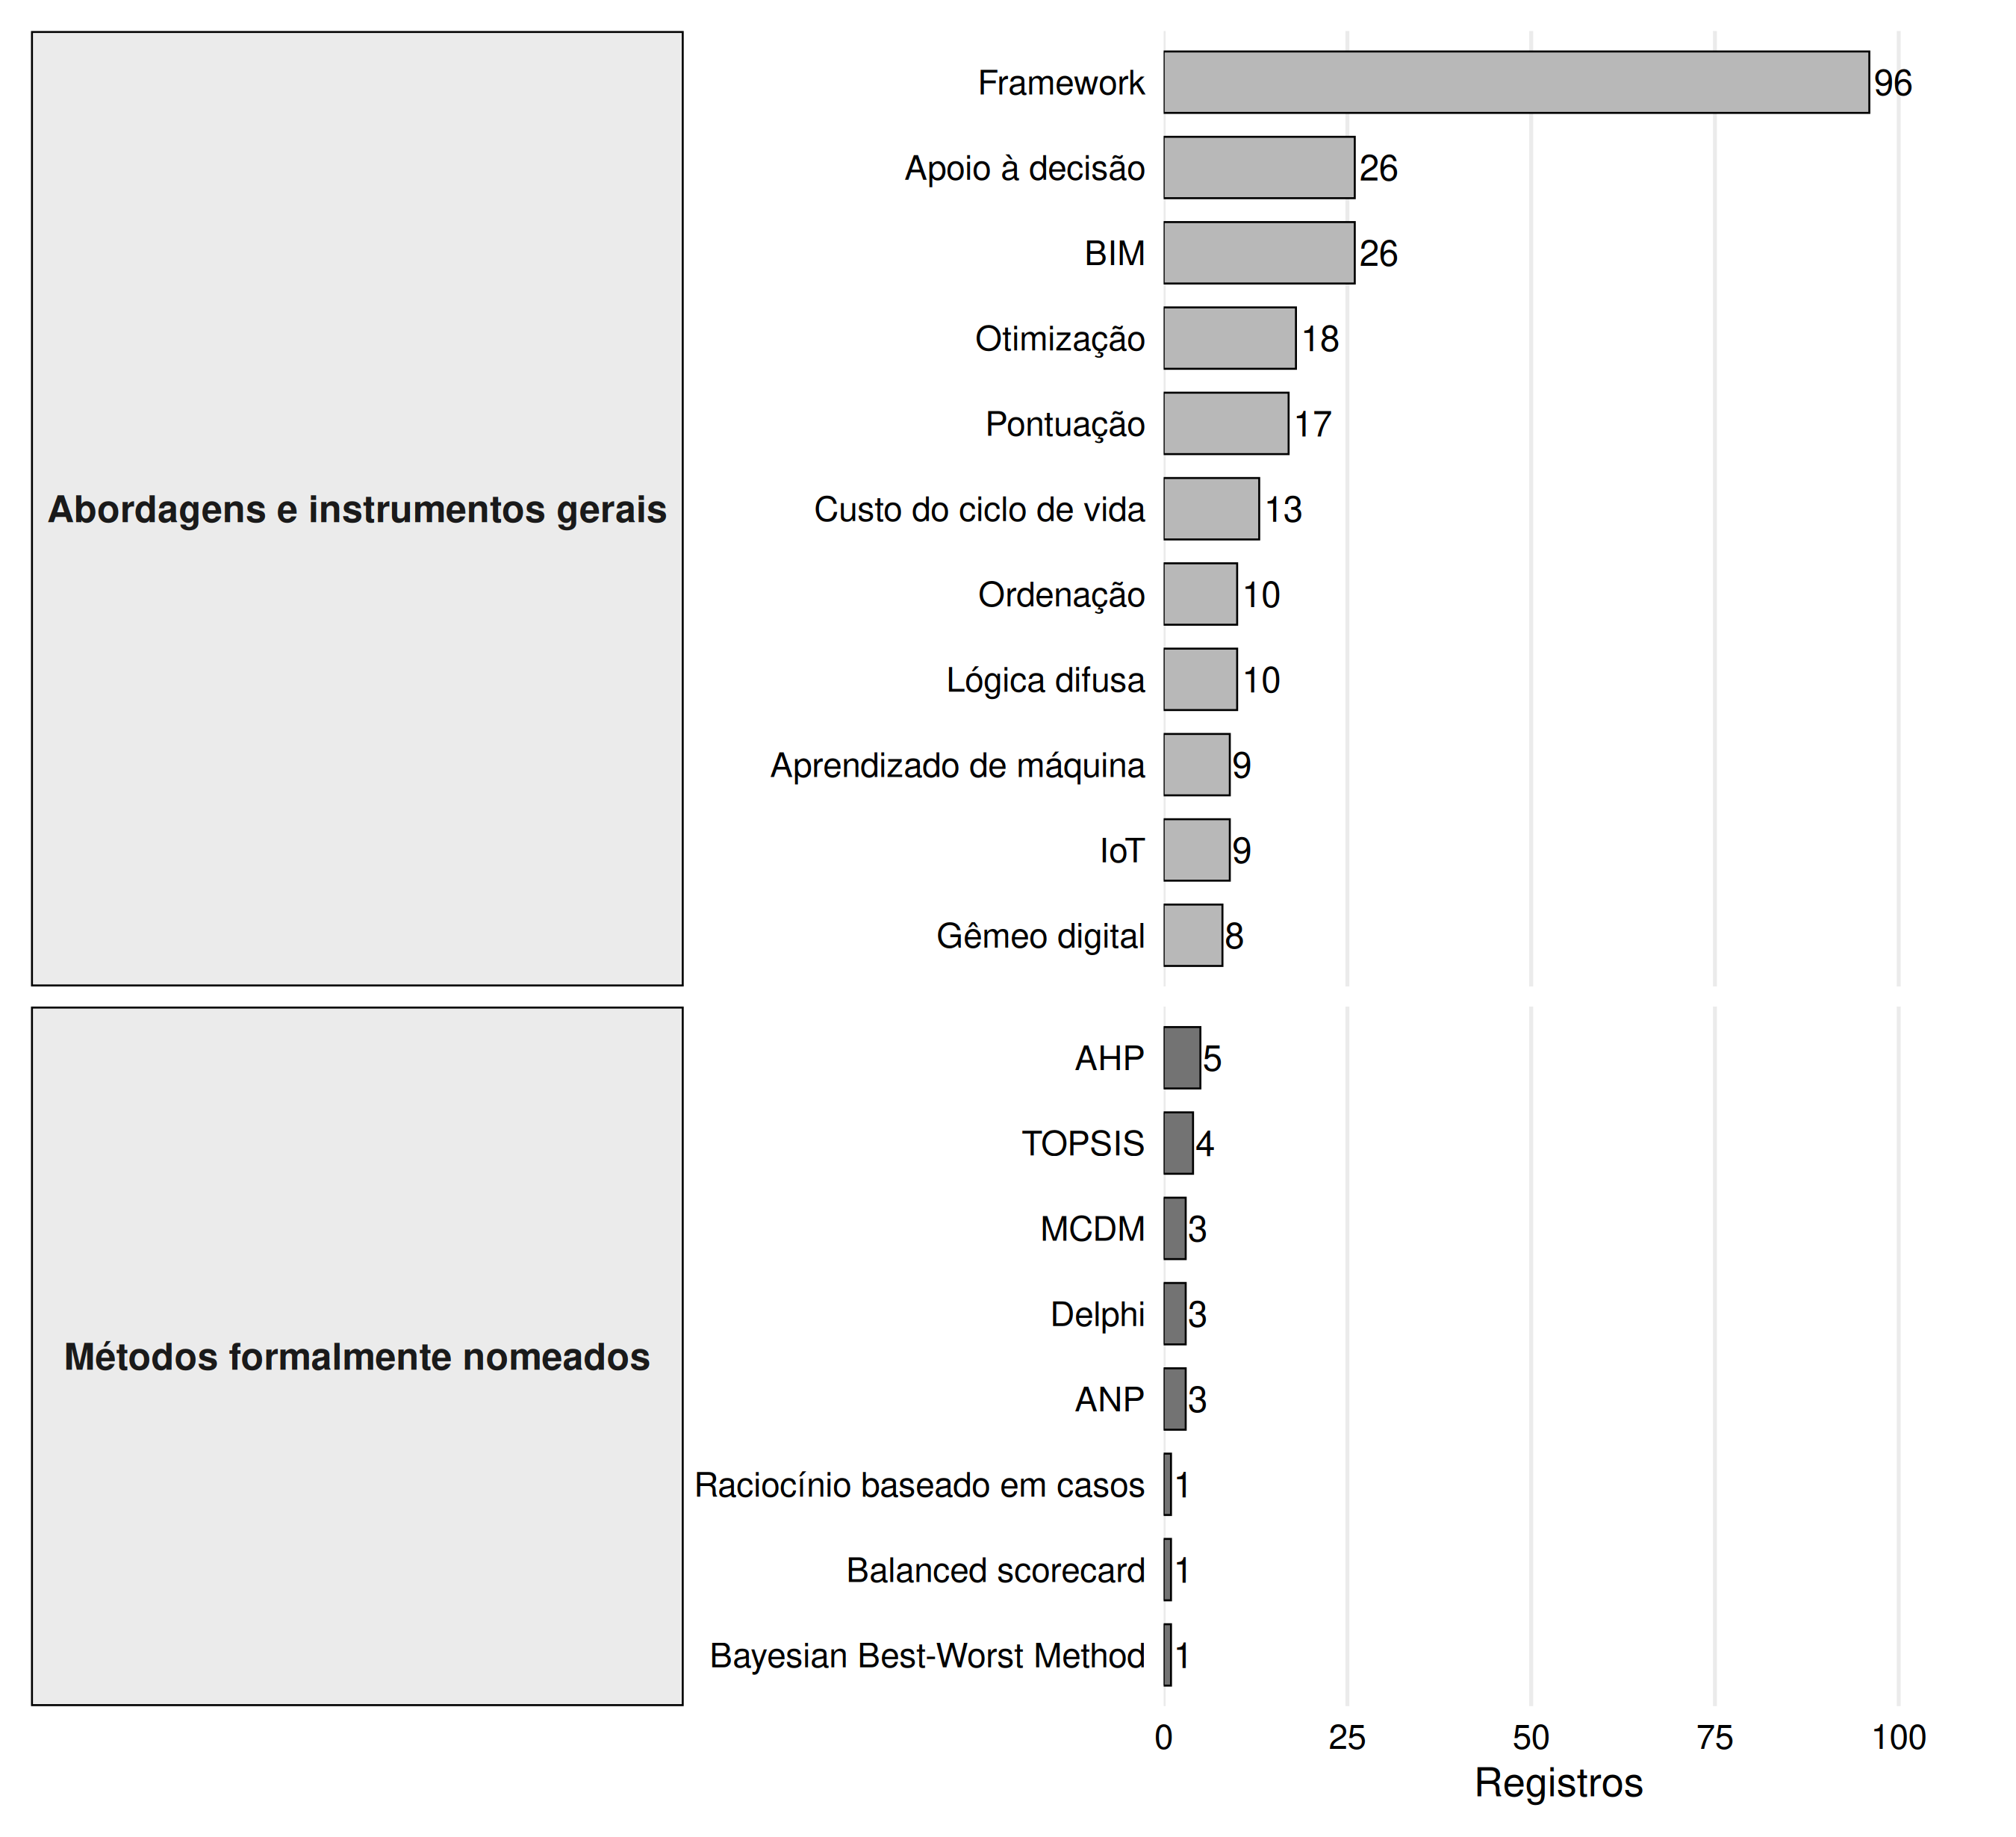
\includegraphics[width=0.95\linewidth]{figuras/figura11_metodos_mcdm_mais_frequentes_nucleo_final_104.png}
\captiongrafico{Abordagens e métodos de apoio à decisão identificados no núcleo final}
\label{fig:metodos}
\end{figure}

Os estudos do núcleo ilustram diferentes formas de estruturar a decisão. O modelo de \textcite{alfalah_frameworkeducacional_2022} combina avaliação de sustentabilidade e ANP difuso em edifícios de ensino. \textcite{naji_campusdelphi_2023} utilizam Delphi modificado para desenvolver um referencial operacional de gestão de facilidades em \textit{campus}. \textcite{masmoudi_ahptopsis_2026} integram AHP, TOPSIS e otimização na alocação de prestadores para manutenção de edifícios públicos. Em conjunto, essas aplicações mostram que os métodos podem organizar critérios técnicos, econômicos, ambientais e sociais em diferentes problemas de gestão predial.


\section{Aplicabilidade a edificações públicas universitárias}
\label{sec:aplicabilidade}

A caracterização documental identificou 93 registros sobre edificação genérica e 58 sobre portfólio predial. Entre as tipologias específicas, houve 17 registros sobre hospitais, 15 sobre edifícios comerciais, 12 residenciais, 11 universidades, dez \textit{campus}, cinco edifícios públicos, cinco escolas, quatro patrimônios históricos e um museu. As categorias são respostas múltiplas; edificação genérica é uma categoria-guarda-chuva, não uma tipologia homogênea.

\begin{table}[H]
\centering
\caption{Contextos de edificação identificados no núcleo final}
\label{tab:contexto}
\small
\begin{tabularx}{\textwidth}{Y >{\raggedleft\arraybackslash}p{2.1cm} >{\raggedleft\arraybackslash}p{2.1cm}}
\toprule
Contexto & Registros & \% dos 104 \\
\midrule
Edificação genérica & 93 & 89,4 \\
Portfólio predial & 58 & 55,8 \\
Hospital & 17 & 16,3 \\
Edifício comercial & 15 & 14,4 \\
Edifício residencial & 12 & 11,5 \\
Universidade & 11 & 10,6 \\
\textit{Campus} & 10 & 9,6 \\
Edifício público & 5 & 4,8 \\
Escola & 5 & 4,8 \\
Patrimônio histórico & 4 & 3,8 \\
Museu & 1 & 1,0 \\
\bottomrule
\end{tabularx}
\fonteautor
\end{table}

Em instituições de ensino, a gestão sustentável combina desempenho físico, usuários e capacidade administrativa. A literatura identifica fatores críticos em universidades \parencite{awuzie_fmuniversidades_2017}, critérios ambientais, econômicos e sociais em edifícios educacionais \parencite{alfalah_frameworkeducacional_2022}, indicadores operacionais de \textit{campus} \parencite{naji_campusdelphi_2023}, previsão orçamentária e uso de ordens de serviço \parencite{martins_custosmanutencaoses_2024,morais_eficienciamanutencao_2023}. O produto deve, portanto, registrar fonte e data dos dados, ausências, unidade comparada, vetos e histórico de pesos, usando entradas simples e exportáveis para prestação de contas.

A baixa frequência de universidade, \textit{campus} e edifício público confirma a lacuna de validação em portfólios heterogêneos, com restrições orçamentárias, continuidade acadêmica e múltiplos usuários. Em texto completo, a manutenção sustentável foi associada à resiliência institucional e aos ODS 4, 9 e 11 \parencite{ndukuba_resilienciainstitucional_2025}; um instrumento estrangeiro exigiu adaptação e concordância profissional em hospital público \parencite{talib_hospitalfm_2013}; e três projetos mostraram perda de informação na transição entre construção e operação, enfrentada pela integração de BIM, \textit{Soft Landings} e comunicação \parencite{tan_fluxoinformacao_2018}. Esses achados sustentam governança da informação e validação contextual, sem equivaler a validação do protocolo proposto.

\section{Matriz analítica proposta}
\label{sec:matriz}

O Gráfico~\ref{fig:heatmap} apresenta a coocorrência documental entre os dez critérios de priorização e os dez instrumentos de apoio à decisão mais frequentes. Desempenho operacional e \textit{framework} aparecem conjuntamente em 88 registros. Informação e dados apresentam 71 coocorrências com \textit{framework} e 26 com BIM. Custo e \textit{framework} aparecem em 55 registros, enquanto vida útil e custo do ciclo de vida aparecem conjuntamente em 13.

\begin{figure}[H]
\centering

\includegraphics[width=0.98\linewidth]{figuras/figura13_heatmap_criterios_metodos_nucleo_final_104.png}
\captiongrafico{Coocorrência entre critérios de priorização e instrumentos de apoio à decisão}
\label{fig:heatmap}
\end{figure}

O Gráfico~\ref{fig:matrizanalitica} reorganiza a coocorrência pelas cinco dimensões de sustentabilidade usadas na matriz analítica. A dimensão técnica-operacional apresenta 95 coocorrências com \textit{framework}, 26 com \textit{decision support} e 26 com BIM. A dimensão institucional apresenta 86 coocorrências com \textit{framework}, seguida da ambiental com 77, da econômica com 55 e da social com 53.

\begin{figure}[H]
\centering

\includegraphics[width=0.98\linewidth]{figuras/figura14_matriz_analitica_dimensao_metodo_nucleo_final_104.png}
\captiongrafico{Matriz de coocorrência entre dimensões de sustentabilidade e instrumentos de apoio à decisão}
\label{fig:matrizanalitica}
\end{figure}

A matriz analítica resultante combina cinco grupos de critérios. A dimensão ambiental reúne energia, emissões, água e resíduos. A econômica reúne custo de manutenção e custo do ciclo de vida. A social reúne segurança, conforto e satisfação dos usuários. A técnica-operacional reúne desempenho, condição física, vida útil e manutenibilidade. A institucional reúne governança, conformidade, informação e capacidade de execução. As linhas da matriz podem ser ponderadas conforme os objetivos da instituição e relacionadas a métodos de pontuação, AHP, TOPSIS, ANP, otimização ou outras formas estruturadas de apoio à decisão.

As coocorrências representam codificações simultâneas no mesmo registro; não estimam associação estatística, efeito, causalidade, peso ou importância dos elementos. Essa síntese transforma os padrões documentais de coocorrência em uma estrutura para pesquisas aplicadas. Sua utilização em instituições públicas de ensino superior requer definição operacional dos indicadores, regras de normalização, processo transparente de ponderação e validação com dados de manutenção, custos, condição dos ativos e percepção dos usuários.


\section{Limitações}
\label{sec:limitacoes}

\textbf{Cobertura.} O ano de 2026 é parcial e os índices podem mudar. Não houve pré-registro público do protocolo. Também não foram realizadas busca de citações para frente ou para trás nem busca estruturada de literatura cinzenta, e a cobertura permaneceu condicionada às fontes e aos metadados indexados, apesar da ausência de filtros de idioma ou tipo documental.

\textbf{Seleção e codificação.} As decisões de triagem e codificação foram conduzidas por um único avaliador, sem segundo revisor independente e sem medida de concordância interavaliadores, e o codebook e termos amplos, como \textit{framework}, incorporam escolhas analíticas. Presença lexical, variável mensurada, critério aplicado e resultado empírico não são equivalentes; ODS, SDG e ESG podem estar ausentes mesmo quando seus componentes aparecem.

\textbf{Extração e força de evidência.} O núcleo de 104 não foi submetido integralmente a elegibilidade e extração em texto completo. Trinta estudos com PDF disponível foram posteriormente lidos em tarefas pontuais e 14 forneceram evidências específicas. A unidade de análise quantitativa é o registro bibliográfico consolidado. Ela não garante independência entre publicações relacionadas nem representa força de evidência acumulada; a classificação de desenho deixou 23,1\% sem sinal suficiente e nenhum instrumento de risco de viés foi aplicado, o que impede comparar qualidade metodológica ou recomendar superioridade.

\textbf{Bibliometria.} Pela incompletude de autores e pela ausência de afiliações e referências citadas nos 372 registros (Seção~\ref{sec:bibliometriaampliada}), colaboração e acoplamento bibliográfico não foram executados; mapa temático, evolução e coocorrências permanecem explorações documentais, sem direção causal ou peso científico.

\textbf{Protocolo.} Indicadores e regras formam especificação operacional candidata: pesos, limiares, função de agregação e sensibilidade ainda não foram validados nem executados com dados reais, permanecendo dependentes de validação de conteúdo, participação institucional e teste de robustez.

\section{Considerações finais}
\label{sec:consideracoes}

A pergunta central foi respondida pela integração de duas camadas parcialmente sobrepostas. O mapeamento bibliométrico identificou transição de eficiência, desempenho e edificações verdes para BIM, \textit{digital twins}, carbono, ciclo de vida e manutenção preditiva. A síntese temática mostrou que dimensões técnica-operacional, institucional e ambiental e critérios de desempenho, informação, custo, vida útil, energia e risco formam o núcleo documental. Dos 121 registros temáticos, 109 também pertencem ao estrato bibliométrico de 372. Essa integração fundamentou a matriz de critérios e indicadores e o fluxo de validação para futura parametrização multicritério.

Foram identificadas seis dimensões, 15 critérios e abordagens decisórias heterogêneas. Estruturas genéricas, BIM e apoio à decisão foram mais frequentes que métodos multicritério nomeados. A busca de sensibilidade elevou o aprendizado de máquina de nove para 26 registros. Entre os 17 incorporados, dez concentram-se em previsão ou previsão com otimização, dois em diagnóstico e classificação e cinco em síntese ou integração tecnológica. Em conjunto, eles cobrem partes da cadeia entre modelo treinado, validação externa, ponderação, vetos e decisão pública auditável.

Edificações genéricas e portfólios predominaram, enquanto universidades, \textit{campus} e edifícios públicos foram menos frequentes. Doze registros apresentaram lacunas específicas para instituições públicas de ensino superior, resultado detalhado na Seção~\ref{sec:aplicabilidade}. Os ODS apareceram em um registro, e os componentes ambientais, sociais e institucionais foram mais frequentes que o rótulo ESG \parencite{masmoudi_ahptopsis_2026,ramantswana_esgfm_2026}.

A contribuição central é uma especificação operacional candidata e rastreável. A revisão sustenta os critérios; indicadores, unidades, fontes, periodicidades e direções são proposições autorais para validação. A definição de pesos, agregação, limiares e vetos integra a etapa institucional seguinte. Quatro frentes organizam essa continuidade:

\begin{enumerate}
\item \textbf{Validação de conteúdo:} painel de manutenção, engenharia, sustentabilidade, planejamento, orçamento e usuários revisa dimensões, indicadores e vetos antes da elicitação dos pesos.
\item \textbf{Integração de dados:} ordens de serviço, inspeções, custos, consumo, riscos e reclamações recebem dicionário, periodicidade e responsáveis.
\item \textbf{Construção de protótipo:} método de elicitação, normalização, pesos, agregação, limiares, casos retrospectivos e análise de sensibilidade são parametrizados e testados.
\item \textbf{Validação multicampi:} estabilidade, utilidade decisória e transferência são comparadas entre unidades e outros portfólios públicos.
\end{enumerate}

Diante da escassez de recursos, esta especificação oferece um caminho para justificar cada investimento por critérios documentados e auditáveis, convertendo a priorização da manutenção de resposta improvisada em prática de governança e valor público.

\nocite{abnt_nbr14037_2011}
\nocite{abnt_isso41001_2020}

\printbibliography[title={Referências}]

\end{document}
